\documentclass{article}
\usepackage[utf8]{inputenc}
\usepackage{graphicx}

\title{ Wiki Distribué } 
\author{ Erick Lavoie \\ Frédéric van der Essen}



\begin{document}
	\maketitle
	\section{Mode d'emploi} 
	\begin{figure}[h]
		\centering
		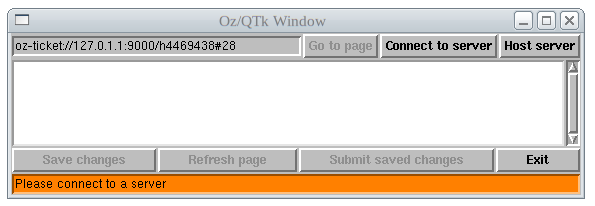
\includegraphics[scale=0.5]{connection.png}
		\caption{L'application en phase de connection}
	\end{figure}
	\begin{figure}[h]
		\centering
		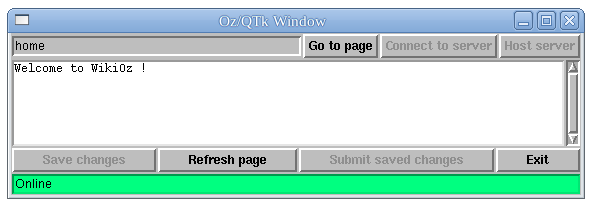
\includegraphics[scale=0.5]{connected.png}
		\caption{L'application en phase de navigation}
	\end{figure}
	
	\subsection{Se connecter au réseau}
	La première étape lorsque l'on ouvre le programme est de se connecter
	à un réseau pair à pair. Notre implémentation permet à l'utilisateur de
	choisir deux options. 
	
	\emph{Host Server} initialise un nouveau réseau
	pair à pair avec un nombre suffisants de noeuds pour que celui ci puisse
	fonctionner correctement. Ensuite, l'application s'y connecte et renvoie
	à l'utilisateur un ticket oz pour que d'autres applications puissent s'y
	connecter. Dans ce cas l'ensemble du réseau pair à pair tourne dans
	un seul processus.
	
	\emph{Connect to Server} se connecte à un réseau pair à pair existant.
	Pour ce faire, l'utilisateur doit disposer d'un ticket oz. Si un serveur
	tourne déjà sous le même utilisateur Unix, alors l'application ira
	automatiquement chercher le ticket dans un fichier se trouvant dans
	le répertoire utilisateur. Sinon, l'utilisateur devra trouver son ticket
	oz par mail ou sur un site web. 
	
	Une fois connecté, l'utilisateur peut en appellant \emph{Host Server}
	récupérer un ticket oz vers son client pour que d'autres utilisateurs
	puissent se connecter au réseau via sa machine. 
	
	\subsection{Navigation des pages web}
	Une fois connecté à un réseau, l'utilisateur entre sur la page par défaut
	\emph{home}. L'utilisateur peut se rendre sur n'importe quelle page en
	entrant son url dans la barre du haut. Si cette page n'existe pas, 
	une nouvelle sera automatiquement créée. l'url n'a pas de format spécifique
	et peut être n'importe quelle string. 
	
	L'utilisateur peut aussi rafraichir une page ce qui lui permet d'accéder
	à la dernière version.
	
	\subsection{Édition des pages web}
	Lorsque l'utilisateur est sur une page, il peut la modifier à loisir.
	Pour cela il suffit de l'editer. Après chaque changement dans un paragraphe,
	l'utilisateur doit les sauvegarder. Une fois tous ses changements
	effectués et sauvegardés il peut les envoyer sur le réseau. En cas
	de conflit dans un paragraphe, les changements ne sont pas effectués,
	l'utilisateur est notifié, et la page est rafraichie à sa version la plus
	récente. 
	
	\section{Validation des requis}
	Les deux tests présentés ci-après montrent la gestion des différentes modifications,
	lors d'un conflit et lors d'une modification concurrente réussie.
	
	\subsection{Gestion d'un conflit d'édition}
	Le plus simple cas pour réaliser un conflit d'édition est de suivre les étapes suivantes:
	\begin{itemize}
		\item Démarrer un premier client
		\item Démarrer l'anneau de noeuds ''server'' sur un des deux clients.
		\item Démarrer un deuxième client et se connecter au premier.  Par défaut, le ticket
			du premier sera déjà dans la barre d'adresse.
		\item Sur le premier client, modifier la ligne de texte, sauvegarder et soumettre les
			changements.
		\item Sur le deuxième, modifier également le texte, sauvegarder et soumettre le texte. 
			Le client notifiera que la modification ne peut être effectuée et chargera la dernière
			page valide sur le serveur.	
	\end{itemize}
	
	\subsection{Gestion de modifications concurrentes indépendantes}
	Le plus simple cas pour constater l'intégration de modifications concurrentes est de suivre les étapes suivantes:
	\begin{itemize}
		\item Démarrer un premier client
		\item Démarrer l'anneau de noeuds ''server'' sur un des deux clients.
		\item Démarrer un deuxième client et se connecter au premier.  Par défaut, le ticket
			du premier sera déjà dans la barre d'adresse.
		\item Sur le premier client, ajouter un paragraphe en dessous du premier (actuellement un 
			seul paragraphe peut être ajouté à la fois entre les différentes sauvegarde).
			Sauvegarder et soumettre les modifications.
		\item Sur le deuxième, rafraîchir la page modifiée par le premier client.
		\item Sur le premier client, modifier le premier paragraphe, sauvegarder et soumettre.
		\item Sur le deuxième, modifier le deuxième paragraphe, sauvegarder et soumettre. Les 
			changements effectués sur le premier client vont apparaître.
		\item Rafraîchir la page sur le premier client pour voir apparaître les changements du 
			deuxième client.	
	\end{itemize}
	
	\section{Architecture}
	Le système actuel dédie un noeud par client qui se joint à l'anneau.  Étant donné les différents 
	problèmes de connexion rencontrés, nous nous en sommes tenus à la version simple de l'anneau, 
	sans utiliser la possibilité de ''relaxer'' l'anneau avec des branches.  Pour assurer la majorité lors des
	différentes opérations distribuées, nécessaire pour réaliser les ''commit'' avec l'algorithme Paxos,
	un anneau initial composé de 5 noeuds est initialisé lors que la fonction ''host server'' est utilisée.
	L'anneau tourne alors dans le même processus Oz que le client.  Tous les clients suivants qui
	se connectent auront un noeud dans leur processus qui se connectera au processus initial.  Cette topologie
	a été utlisée pour la simple et unique raison qu'elle minimisait les risques d'erreurs de connexion au moment 
	où un noeud dans un autre processus se joint à l'anneau, puisque plusieurs erreurs ont été 
	rencontrées au courant du développement.
	
	Pour la version finale, nous nous attendions à utiliser un noeud par processus Oz, donc par client et démarrer
	un ensemble de noeuds pour simuler un grand nombre de clients déjà connectés entre eux.  L'objectif final
	serait que même si un client se déconnecte, l'anneau survit et reste intègre.
	
	
	\section{Design}
	Le design du système s'est articulé autour de deux principaux points: la gestion des transactions et le développement
	d'un type de données.
	
	
	\subsection{Limitations}
	 
\end{document}
